% id: 2024-tavares-1-1 | fonte: listas/2024/Tavares/lista2024tavares1.pdf, p. 1
Dada uma configuraçáo com duas cascas esféricas condutoras concêntricas aterradas de raios $a$ e $b$ com $a < b$ e uma carga pontual de valor $q$ a uma distância $a < r < b$, encontre a carga induzida em cada esfera. % sic: "configuraçáo"
\begin{center}
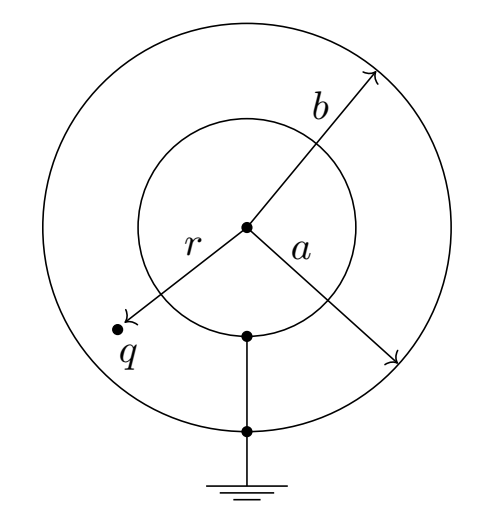
\includegraphics[width=.55\linewidth]{fig/1.png}\\[2pt]
{\small Figura 1: Não pode usar carga imagem!}
\end{center}
